\documentclass[12pt]{article}
\oddsidemargin -0.5in
\evensidemargin -0.5in
\textwidth 7.2in
\topmargin -0.5in
\textheight 8in
\flushbottom

\usepackage[authoryear,round]{natbib} %a package for formatting citations
\usepackage{amsmath} %a package for good looking equations and symbols
\usepackage{algorithm2e} %a package for typesetting algorithms
% \usepackage{caption} %a package for more complex captions for figures/tables/images
\usepackage{subcaption} %extension of the caption package
\usepackage{url} %embedded, clickable links
\usepackage{fullpage} %including this package changes the default margins to use more of the page
\usepackage{graphicx} %package for inline images
\usepackage[usenames]{xcolor} %for adding color text
\usepackage{enumitem} %for nested numbered lists (like in the questions section)
\setlist[description]{style=nextline}
% \usepackage{hyperref}
% \usepackage{amsfonts}

\newcommand{\nextproblem}{
	\vfill
	\pagebreak
}
\setlist[itemize]{noitemsep, topsep=1pt}
\graphicspath{{plots/}}

\begin{document}

\begin{center}
    \textbf{CS 4641 Machine Learning \\ Bojun Yang | Section B Homework 3 Writeup}
\end{center}

\begin{enumerate}[leftmargin=\parindent,align=left,labelwidth=\parindent,noitemsep]
\item \textbf{PCA Analysis}
\begin{itemize}[topsep=10pt]
    \item \textbf{HTRU2} \\
    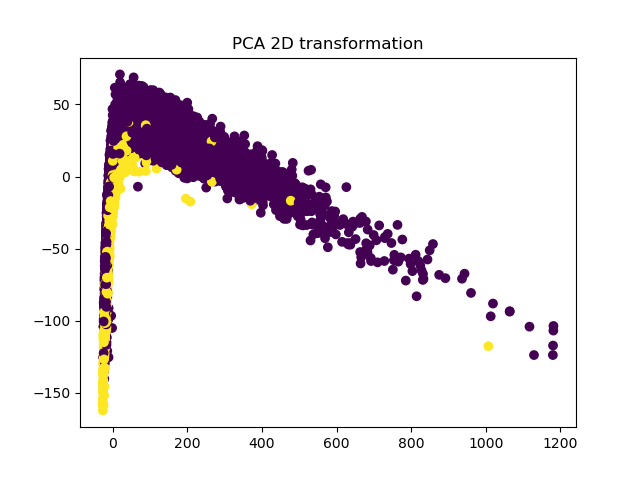
\includegraphics[width=0.45\textwidth]{pca_HTRU2_2d} 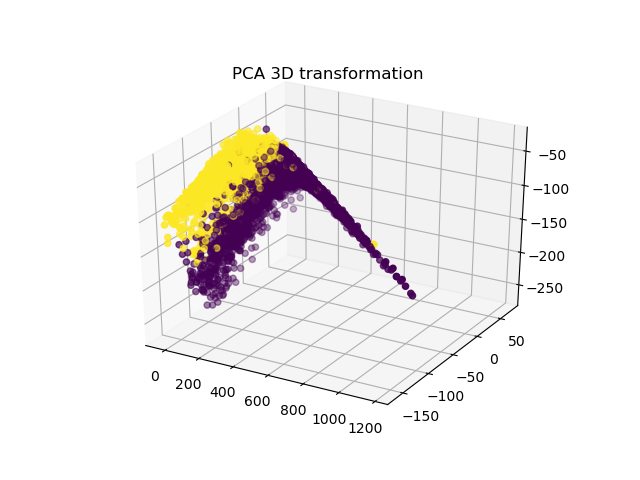
\includegraphics[width=0.45\textwidth]{pca_HTRU2_3d} \\
    It is not apparent that the transformed data is linearly separable from the 2d data of the PCA transformation. It appears that the data set is blended and but there is a separation between the two labels. Taking a look at the 3d data, we can tell that there may exist plane that separates the differently colored data points. \\
    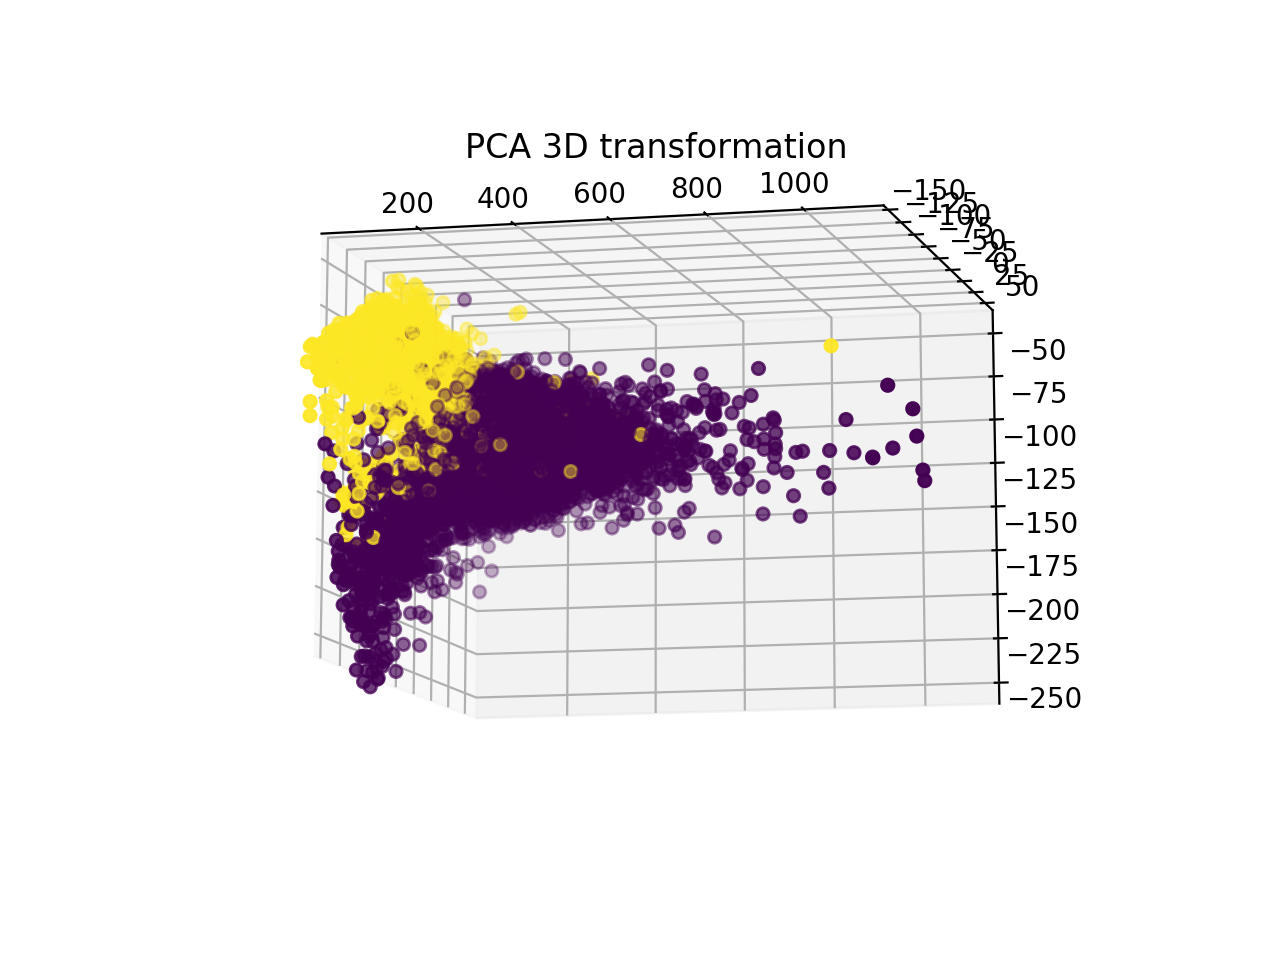
\includegraphics[width=0.55\textwidth]{pca_HTRU2_3d1} \\
    Looking at the 3d data from another angle, we can see another view that also seems to be separable with a plane.
    \begin{itemize}
        \item original data \textbf{fit time}: 0.18409967422485352
        \item 2d transformed data \textbf{fit time}: 0.03162217140197754
        \item 3d transformed data \textbf{fit time}: 0.03455996513366699 \\

        \item 2d \textbf{train} score: 0.9779298784746473
        \item 2d transformed \textbf{train} score: 0.9193323089817014
        \item 3d transformed \textbf{train} score: 0.9709456628020673 \\

        \item 2d \textbf{test} score: 0.9826815642458101
        \item 2d transformed \textbf{test} score: 0.9164804469273743
        \item 3d transformed \textbf{test} score: 0.9745810055865922
    \end{itemize}
    The results of the LogReg tests make sense based on our observations. The 3d transformed data performed better than the 2d transformed data. The performance on the 3d transformed data almost matches the performance on the original data, and a good performance at that. In addition to having similar performance, it is worth noting that the time to fit the data was significantly faster for the transformed data than the original data.
    \item \textbf{digits} \\
    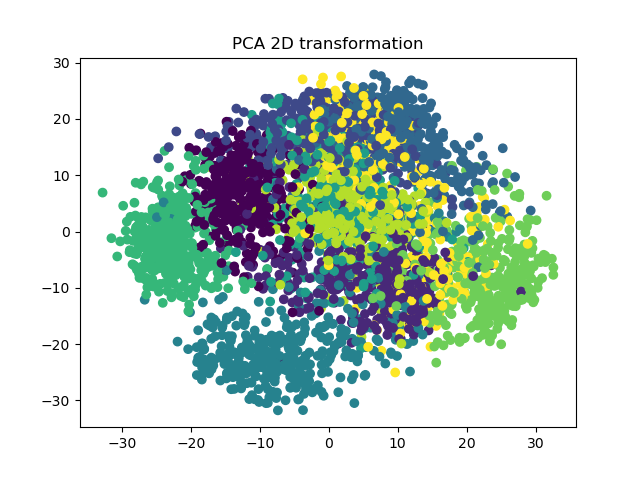
\includegraphics[width=0.45\textwidth]{pca_digits_2d}
    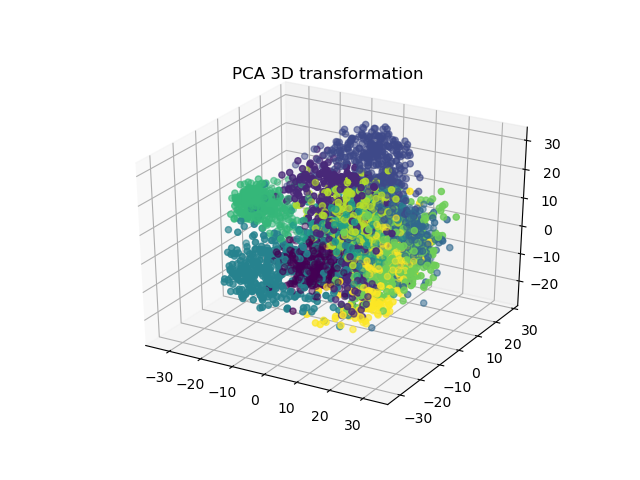
\includegraphics[width=0.45\textwidth]{pca_digits_3d} \\
    It isn't imediately apparent whether the PCA transformed dataset for digits is linearly separable from either the 2d or 3d data. However if we look at the transformed data at different angles in the 3d data as shown below, we can see some separation of the differently colored data points. \\
    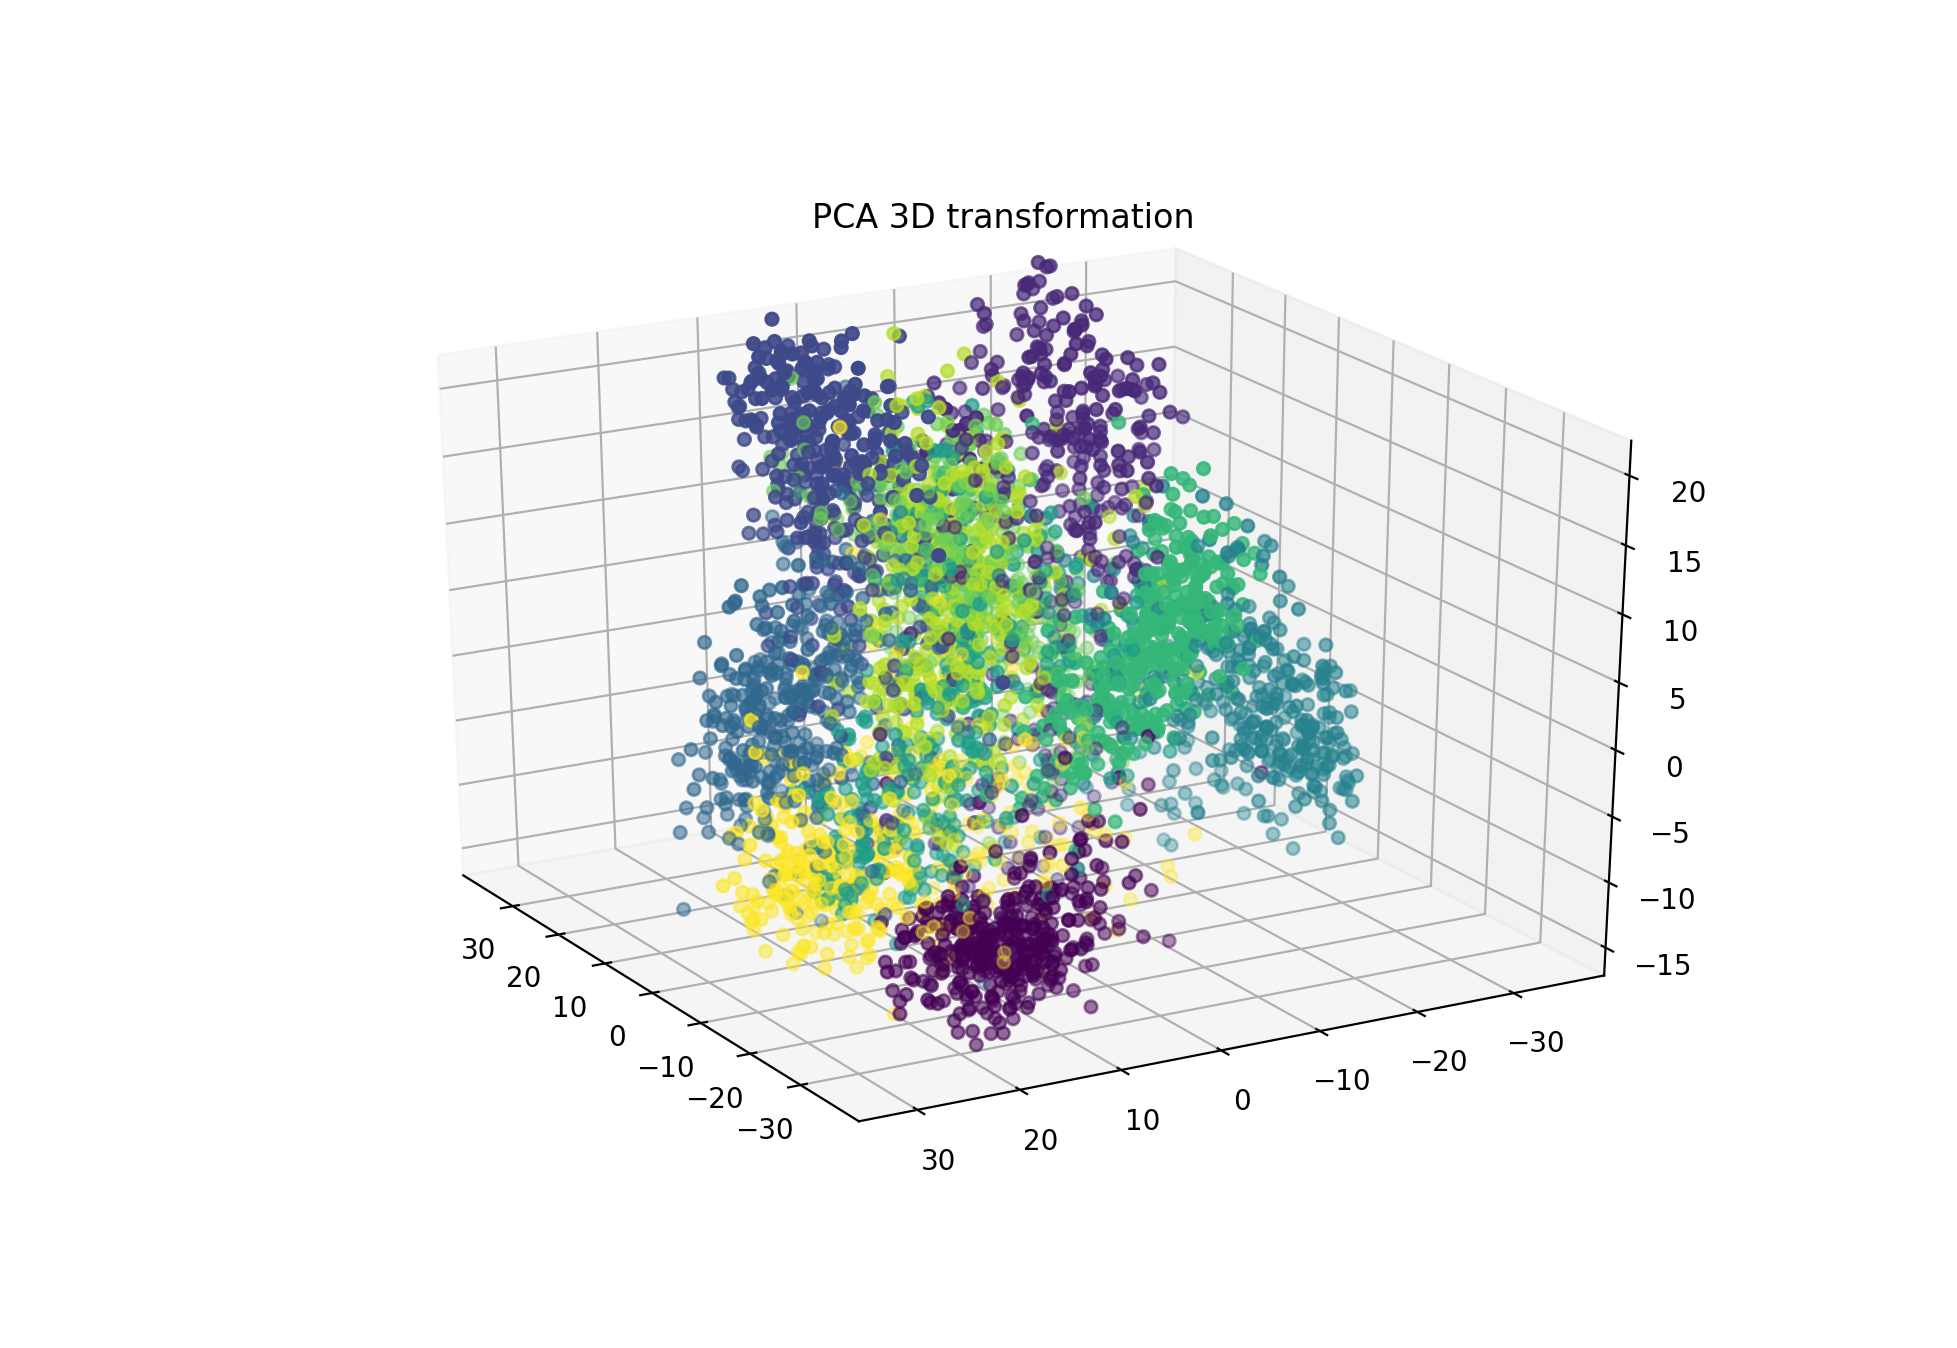
\includegraphics[width=0.35\textwidth]{pca_digits_3d1}
    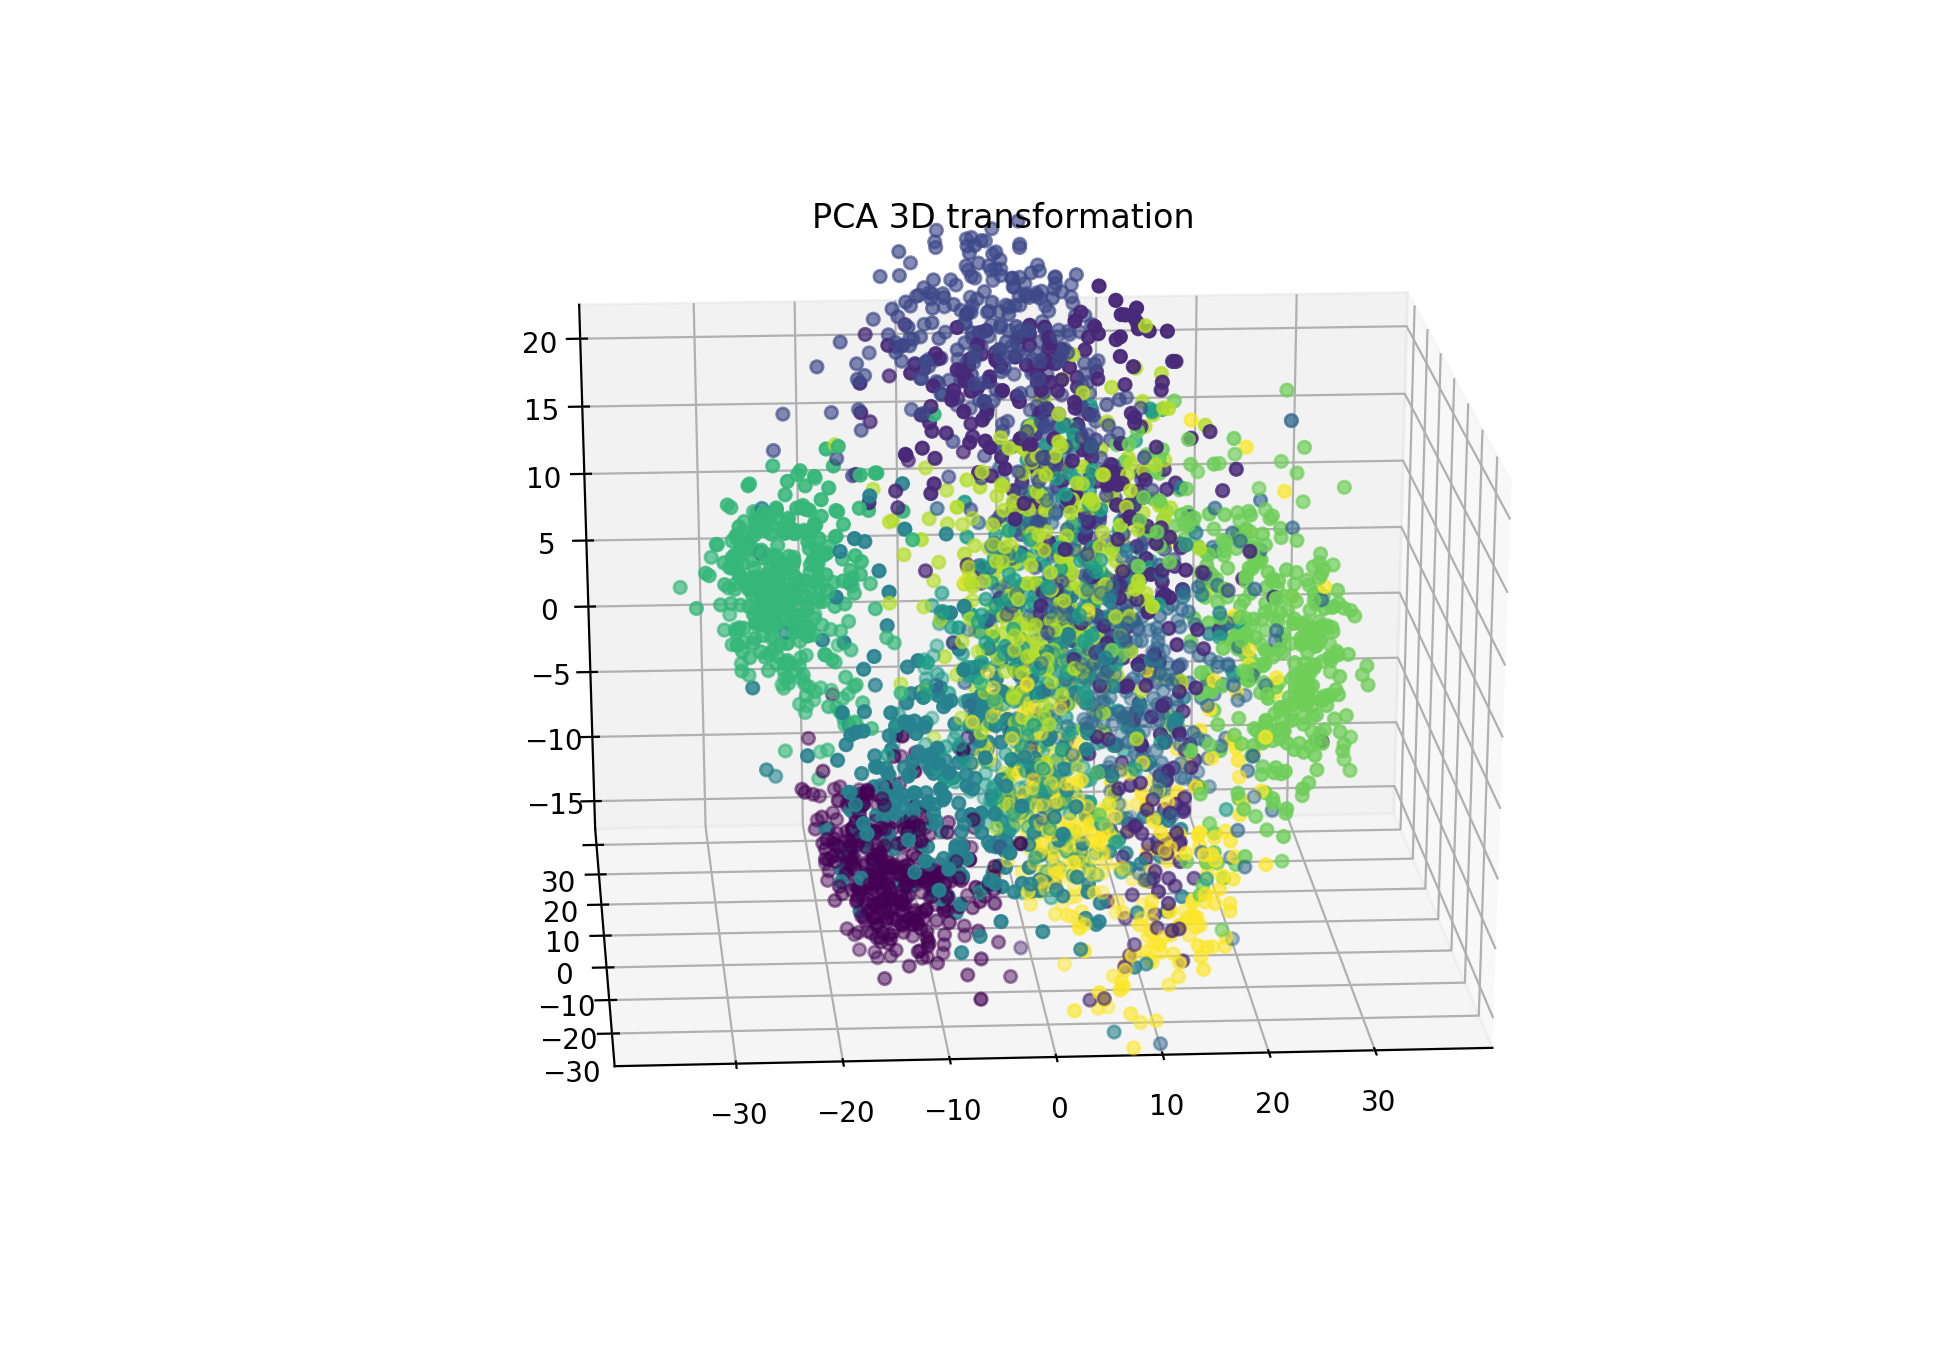
\includegraphics[width=0.35\textwidth]{pca_digits_3d2}
    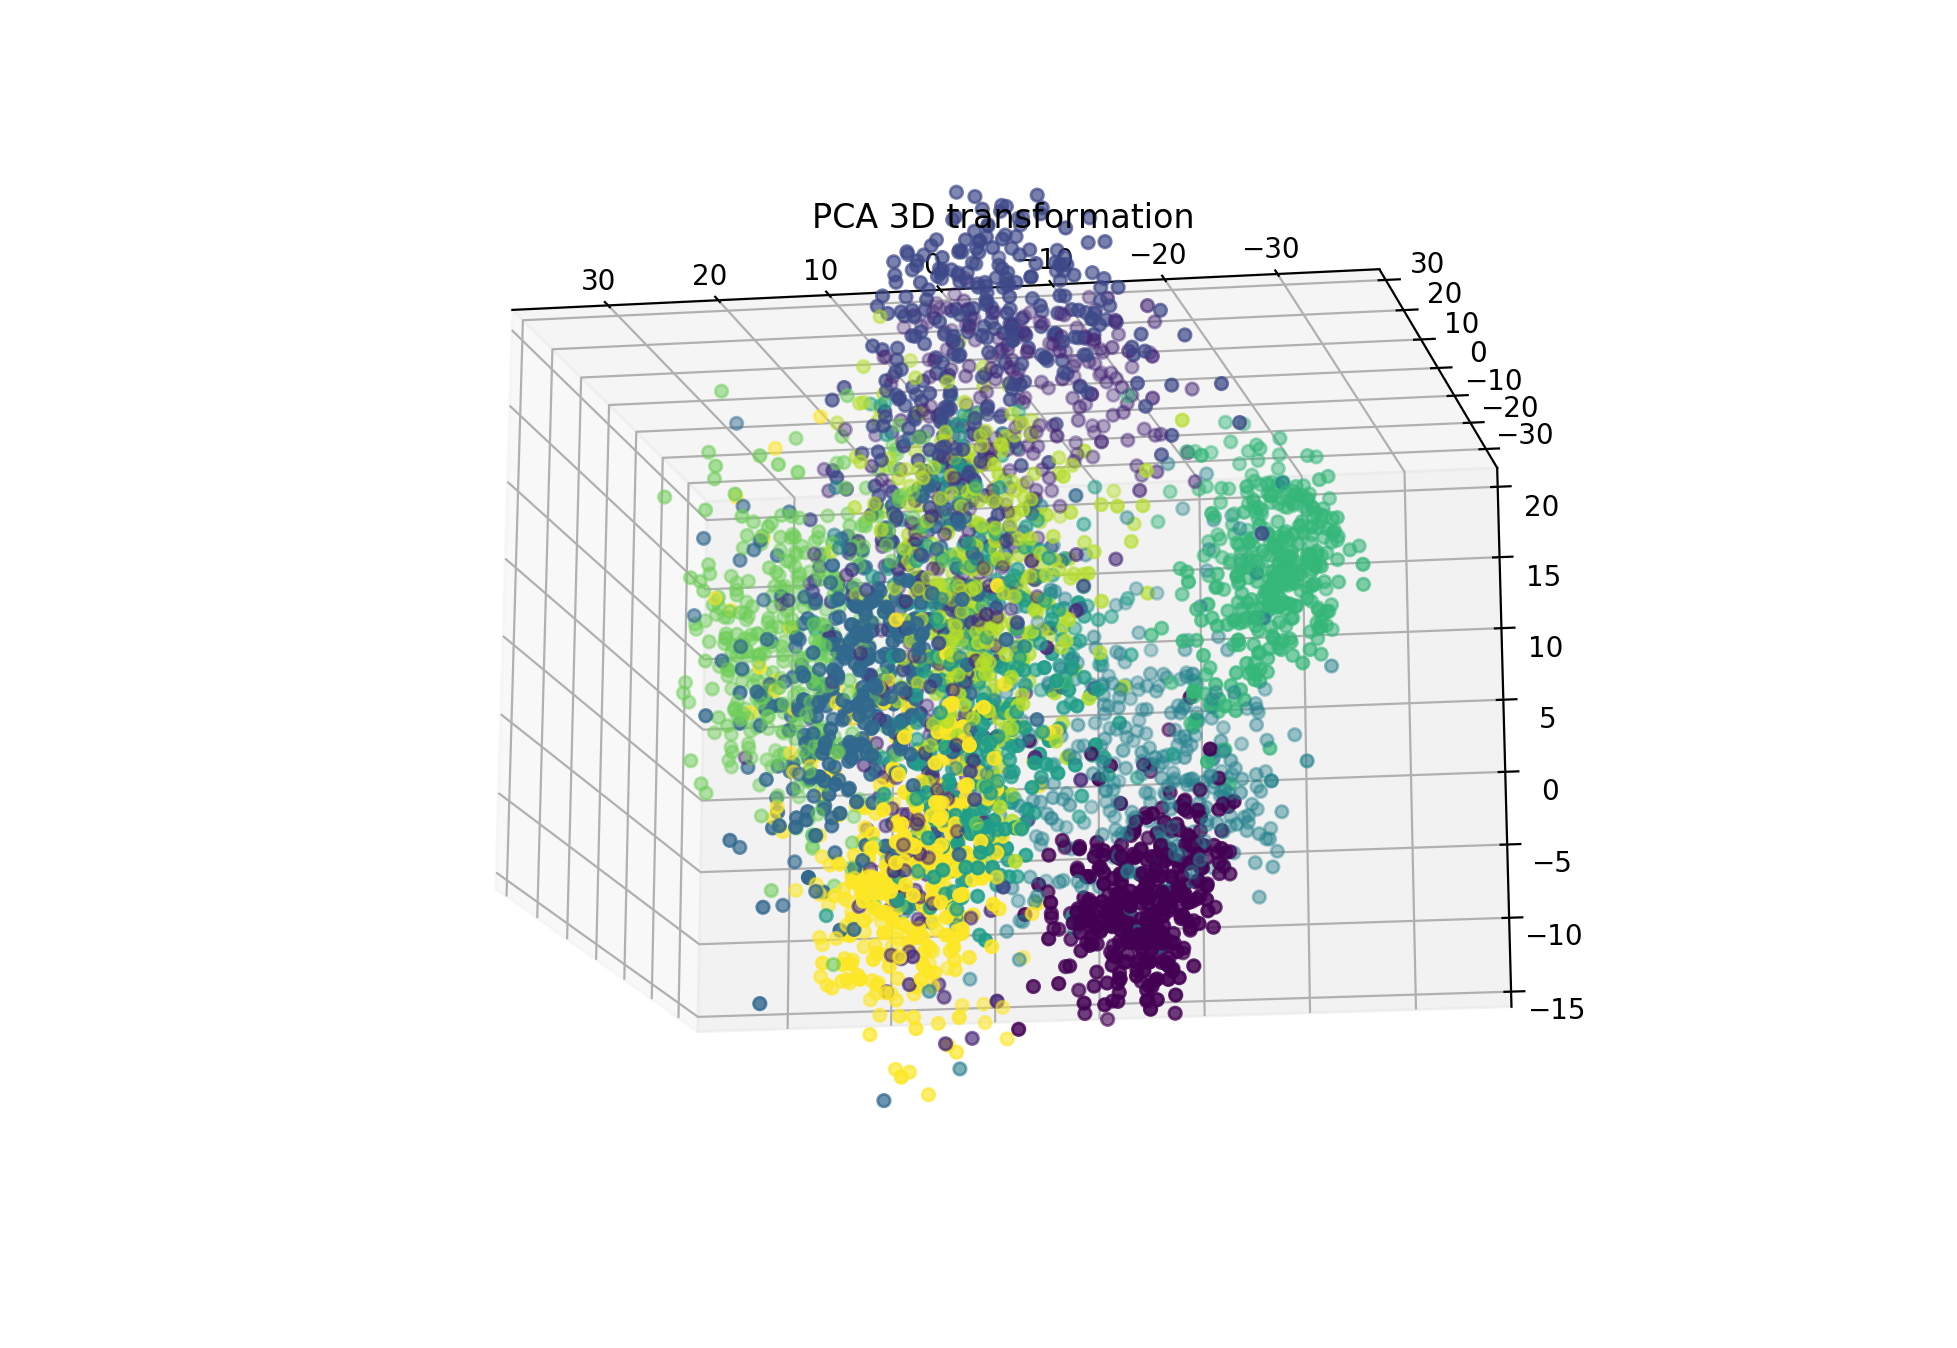
\includegraphics[width=0.35\textwidth]{pca_digits_3d3} \\
    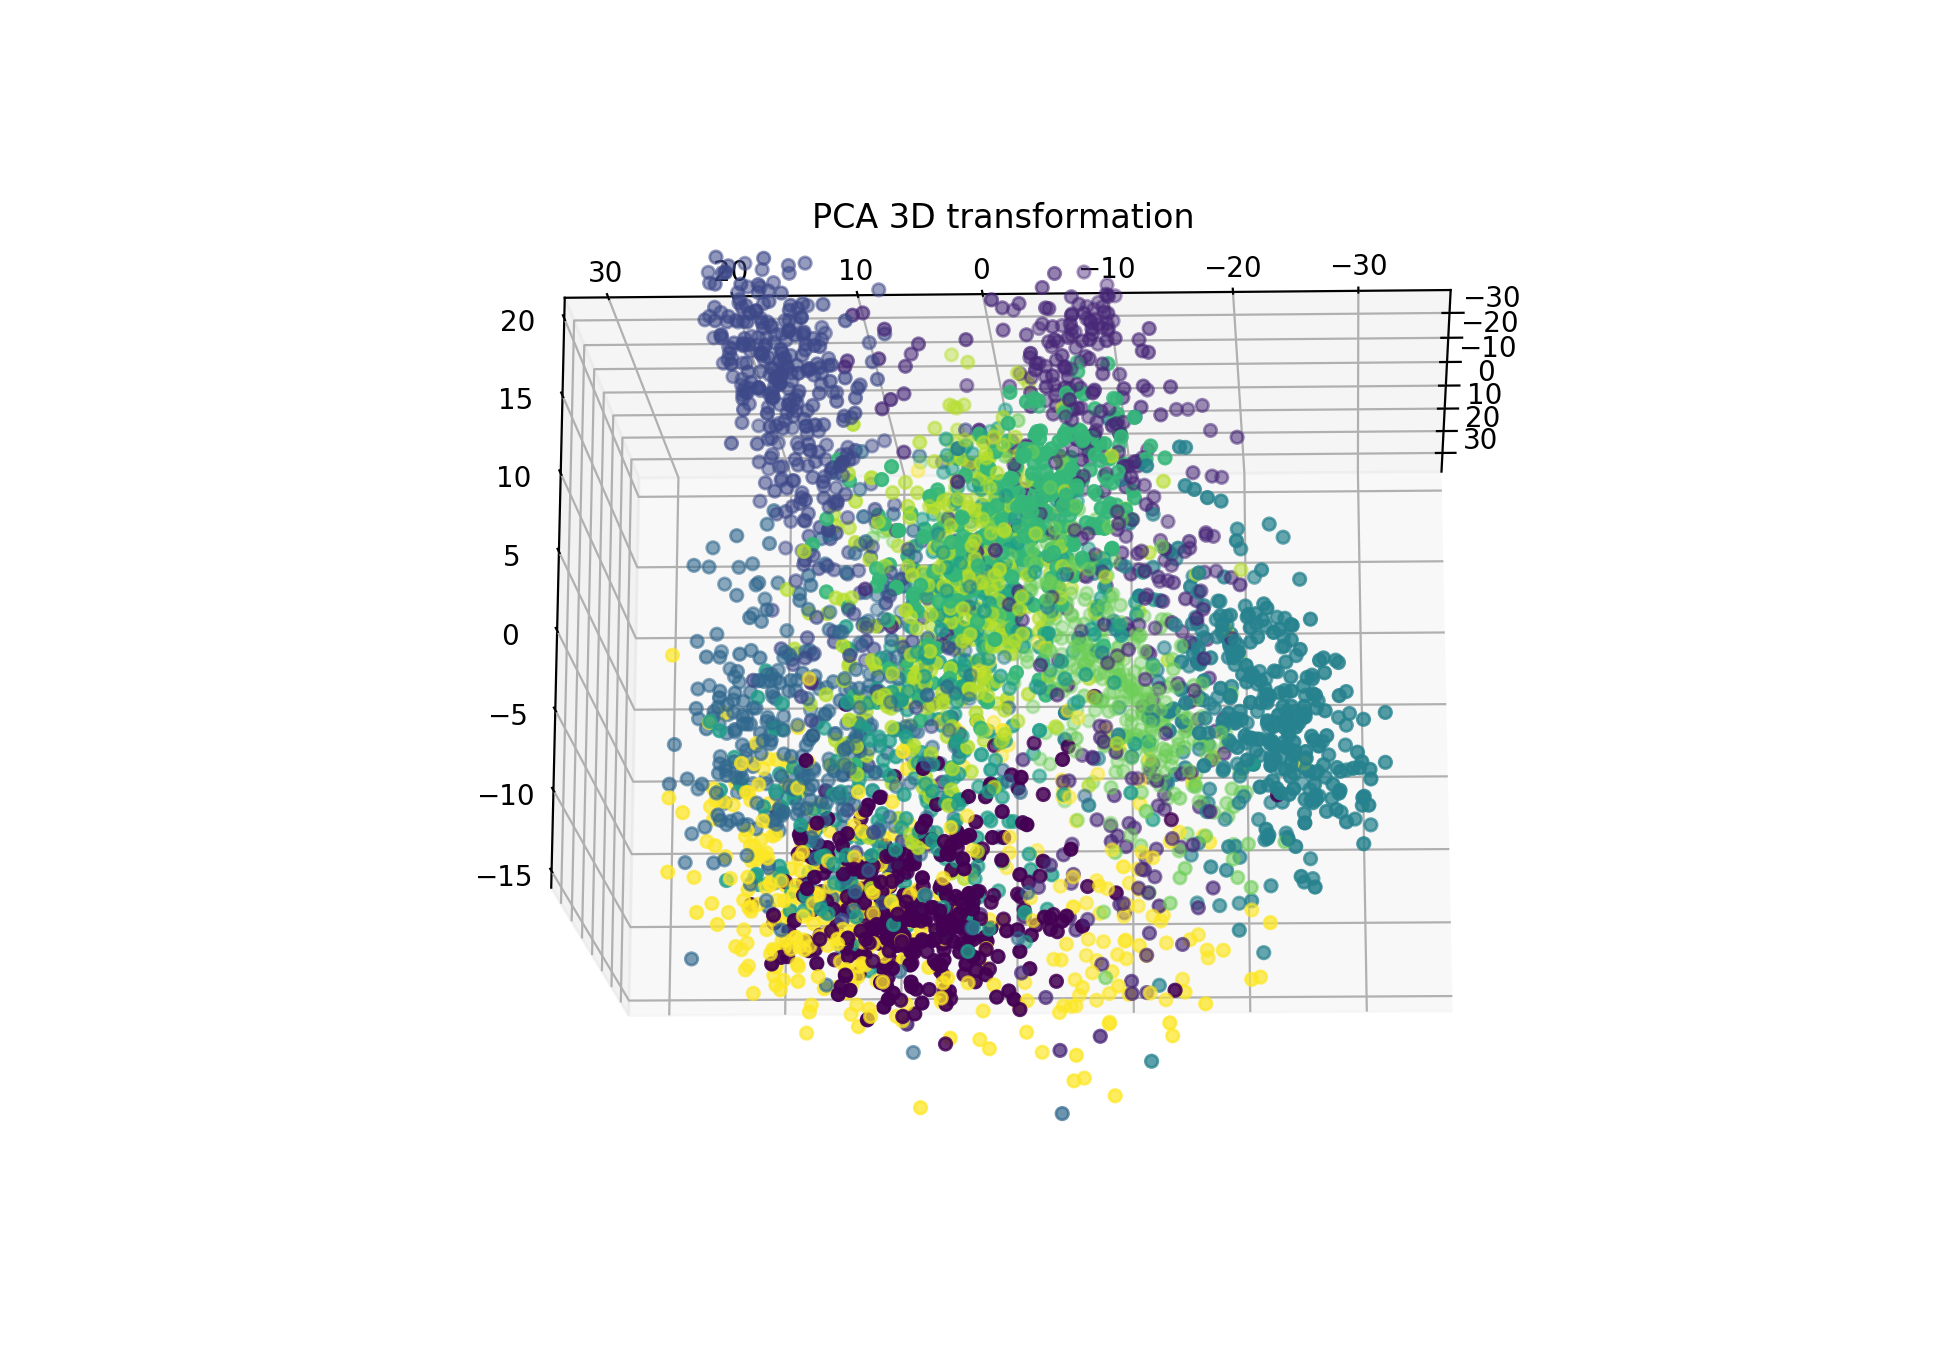
\includegraphics[width=0.35\textwidth]{pca_digits_3d4}
    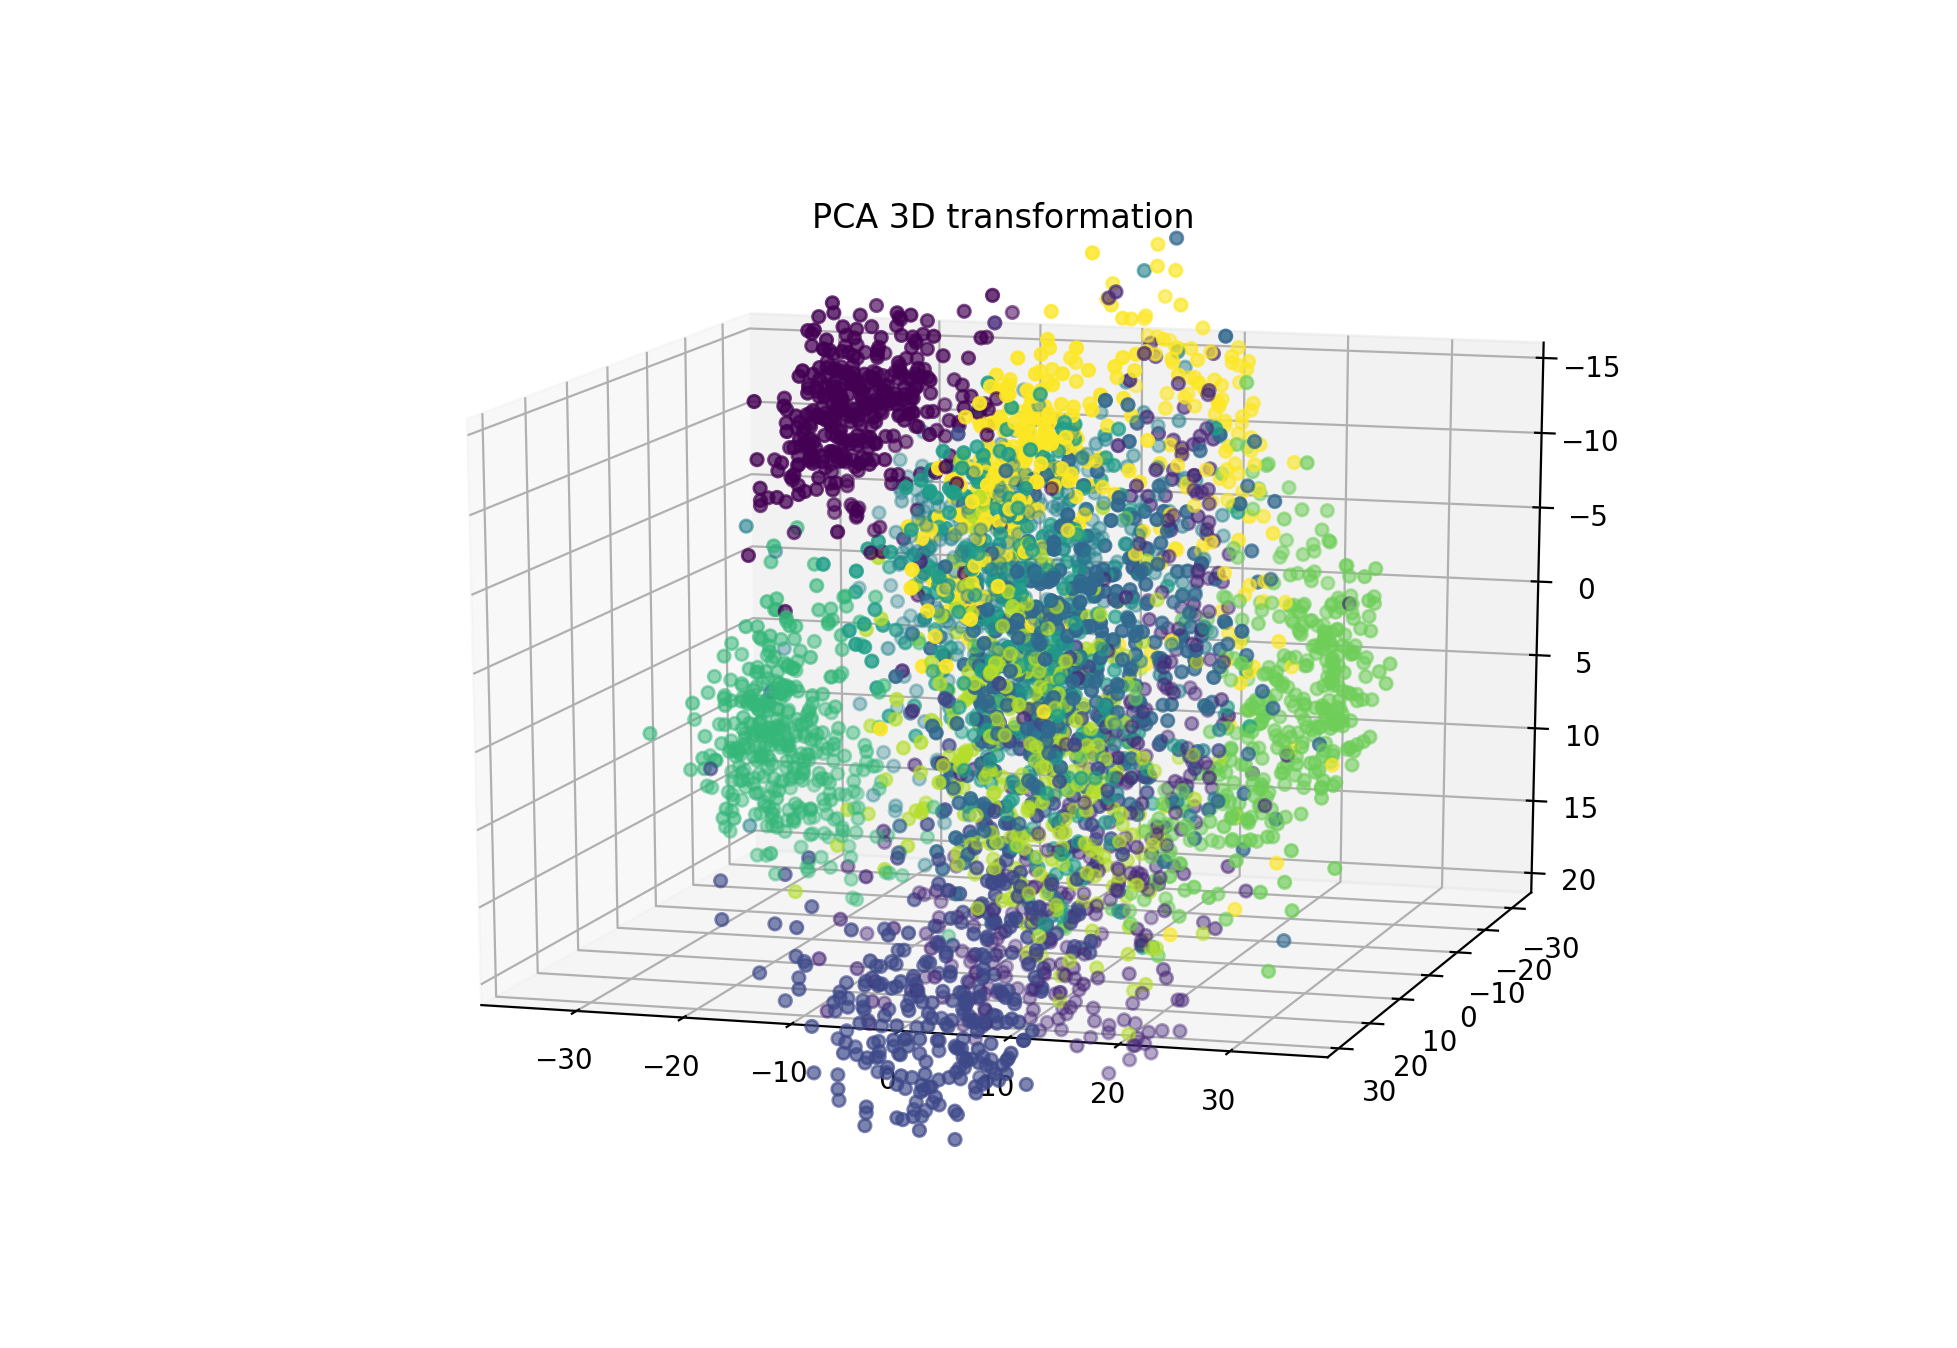
\includegraphics[width=0.35\textwidth]{pca_digits_3d5} \\
    It looks like that all the data groups except for yellow look somewhat linearly separable. However, from the different views, you can tell that the yellow data points form a disk-shaped cloud volume in the middle of the other data points. However, it needs to be noted that each group of points seems overlap with another's groups. \\
    Running LogReg Tests on the data: \\
    \begin{itemize}
        \item original data \textbf{fit time}: 7.577993869781494
        \item 2d transformed data \textbf{fit time}: 0.7825779914855957
        \item 3d transformed data \textbf{fit time}: 0.6092972755432129 \\

        \item 2d \textbf{train} score: 0.999738425320429
        \item 2d transformed \textbf{train} score: 0.612607899555323
        \item 3d transformed \textbf{train} score: 0.7501961810096782 \\
        
        \item 2d \textbf{test} score: 0.9488035614913745
        \item 2d transformed \textbf{test} score: 0.5820812465219811
        \item 3d transformed \textbf{test} score: 0.7089593767390094
    \end{itemize}
    Based on our observations, these results make sense. LogReg did a lot better on the 3d transformed data than the 2d transformed data. However, none of the results from transformed data LogReg were as good as LogReg on the original dataset. These results confirm our suspicion that LogReg will not work well on the transformed data. However, it is worth noticing that the time to fit the transformed data was significantly lower than the time to fit the original data.
    
    \item \textbf{iris} \\
    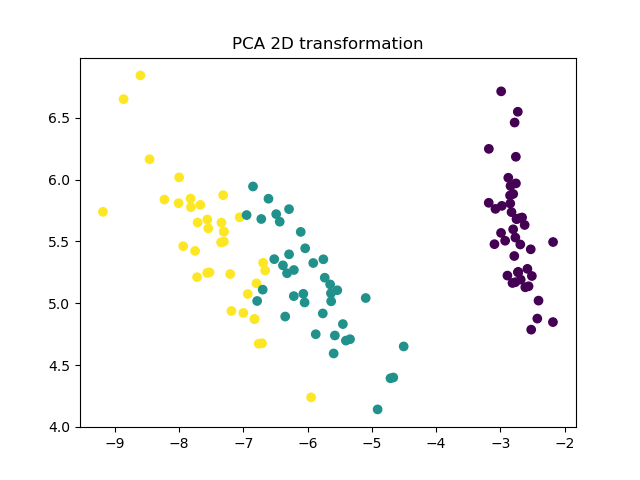
\includegraphics[width=0.45\textwidth]{pca_iris_2d} 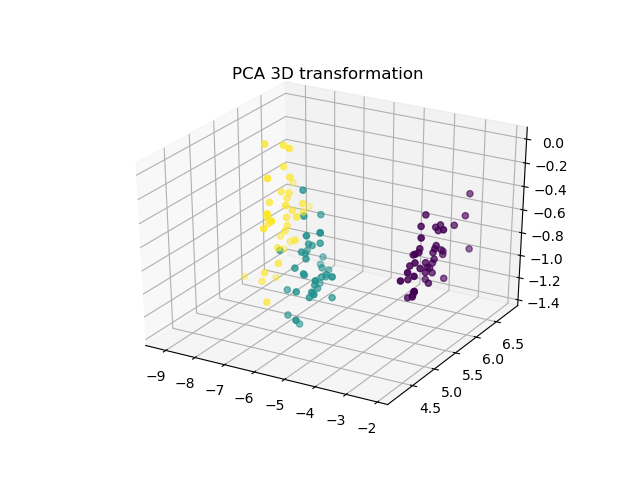
\includegraphics[width=0.45\textwidth]{pca_iris_3d} \\
    From the the 2d and 3d data of the PCA transformation, it is pretty clear that the transformed data is linearly separable. We can see 3 distinct and spearated groups of data points. Therefore, logistic regression will perform well to classify the transformed data.
    \begin{itemize}
        \item original data \textbf{fit time}: 0.041589975357055664
        \item 2d transformed data \textbf{fit time}: 0.011603116989135742
        \item 3d transformed data \textbf{fit time}: 0.01744532585144043 \\

        \item 2d \textbf{train} score: 0.9666666666666667
        \item 2d transformed \textbf{train} score: 0.95
        \item 3d transformed \textbf{train} score: 0.9583333333333334 \\

        \item 2d \textbf{test} score: 0.9666666666666667
        \item 2d transformed \textbf{test} score: 0.9666666666666667
        \item 3d transformed \textbf{test} score: 1.0
    \end{itemize}
    These results confirm our observation that the transformed data will perform well with LogReg. The performances are very similar and within 0.01 difference. 
\end{itemize}

\item \textbf{K-Means Analysis}
\begin{itemize}[noitemsep,topsep=1pt]
    \item \textbf{iris} \\
    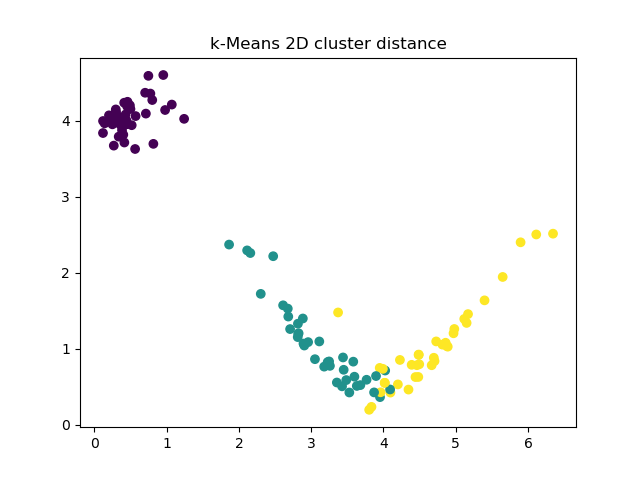
\includegraphics[width=0.45\textwidth]{kmeans_iris_2d} 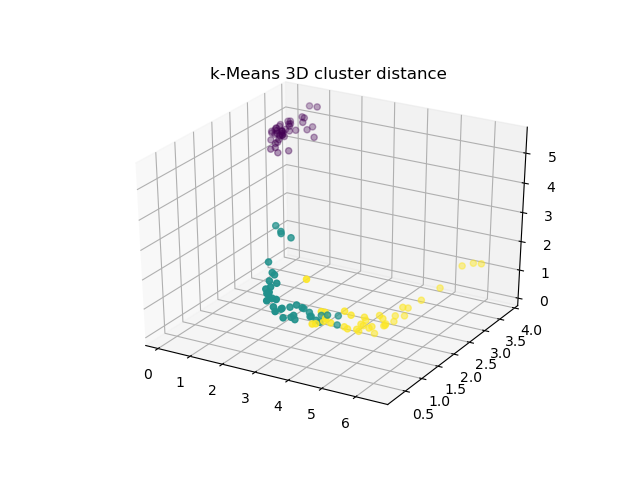
\includegraphics[width=0.45\textwidth]{kmeans_iris_3d} \\
    \begin{itemize}
        \item original data \textbf{fit time}: 0.0294342041015625
        \item 2d transformed data \textbf{fit time}: 0.0076847076416015625
        \item 3d transformed data \textbf{fit time}: 0.014444112777709961 \\

        \item 2d \textbf{train} score: 0.9666666666666667
        \item 2d transformed \textbf{train} score: 0.9416666666666667
        \item 3d transformed \textbf{train} score: 0.9416666666666667 \\

        \item 2d \textbf{test} score: 0.9666666666666667
        \item 2d transformed \textbf{test} score: 0.8333333333333334
        \item 3d transformed \textbf{test} score: 0.8666666666666667 \\
    \end{itemize}
    Using k-Means as a feature transform compared to PCA did not perform as well as PCA. It would be better to use PCA for both 2d and 3d data sets as the performance of PCA transformed data is higher than that of k-Means. The graphs of k-Means on this dataset seems to produce data that is less linearly separable than that of PCA's. \\
    The normalized mutual information was 0.59090106038302613 wtih 3 clusters. This makes sense because NMI is higher when points belonging to the same cluster have the same label. Looking at our graphs of the transformed data, we can imagine three centers where each center's cluster contains mostly purple, green, and yellow points, respectively. 
    \item \textbf{digits} \\
    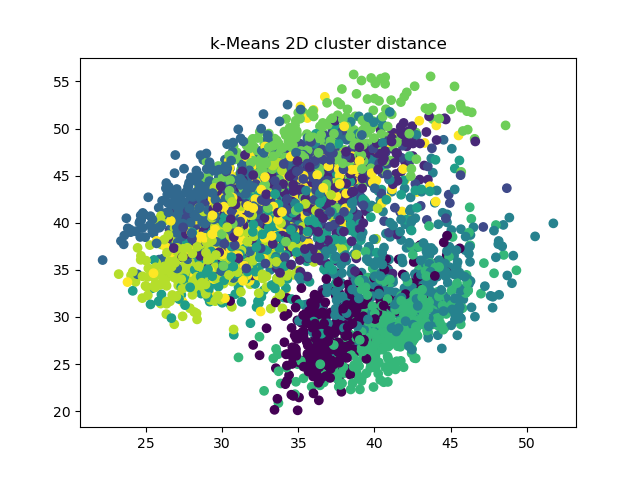
\includegraphics[width=0.45\textwidth]{kmeans_digits_2d} 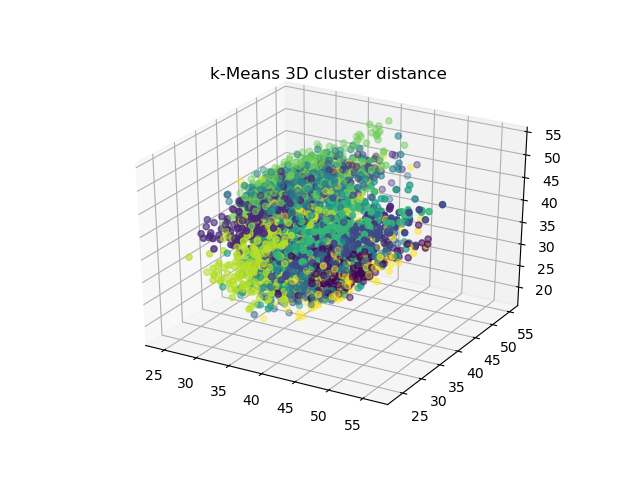
\includegraphics[width=0.45\textwidth]{kmeans_digits_3d} \\
    \begin{itemize}
        \item original data \textbf{fit time}: 6.619047164916992
        \item 2d transformed data \textbf{fit time}: 1.1980550289154053
        \item 2d transformed data \textbf{fit time}: 2.3269810676574707 \\

        \item 2d \textbf{train} score: 0.999738425320429
        \item 2d transformed \textbf{train} score: 0.46089458540413286
        \item 3d transformed \textbf{train} score: 0.4969918911849333 \\
        
        \item 2d \textbf{test} score: 0.9488035614913745
        \item 2d transformed \textbf{test} score: 0.4323873121869783
        \item 3d transformed \textbf{test} score: 0.4802448525319978 \\
    \end{itemize}
    Using k-Means as a feature transform is is not better than PCA. Comparing the LogReg scores with k-Means transformed data against the LogReg score for PCA transformed data, the scores for k-Means transformed is much lower. The graphs of the 2d and 3d data points also confirm this. The data points look to be more clustered together, making it harder for LogReg to find lines/planes of separation. \\
    The normalized mutual information was 0.7449158709032907 with 10 clusters. This makes sense because NMI is higher when points belonging to the same cluster have the same label. The graphs of the transformed data show points that can be sectioned of into 10 different volumes. It's easy to see that each cluster will correspond to one color of points.
    \nextproblem
    \item \textbf{HTRU2} \\
    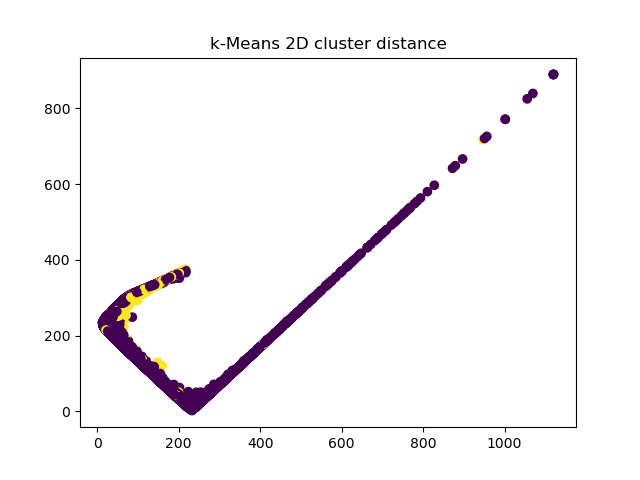
\includegraphics[width=0.45\textwidth]{kmeans_HTRU2_2d} 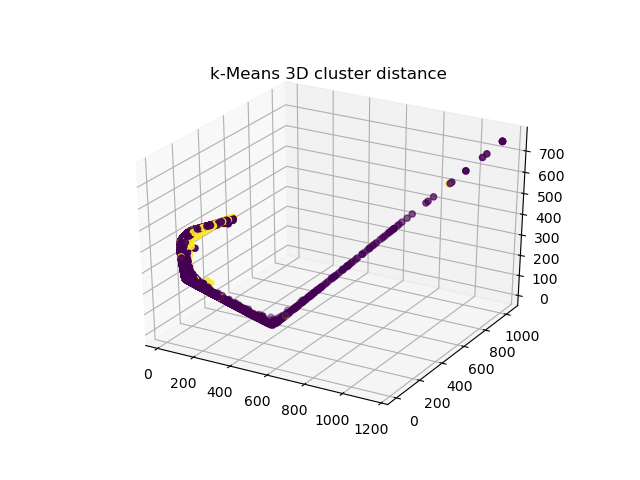
\includegraphics[width=0.45\textwidth]{kmeans_HTRU2_3d} \\
    \begin{itemize}
        \item original data \textbf{fit time}: 0.1594712734222412
        \item 2d transformed data \textbf{fit time}: 0.030047178268432617
        \item 2d transformed data \textbf{fit time}: 0.04154205322265625 \\

        \item 2d \textbf{train} score: 0.9779298784746473
        \item 2d transformed \textbf{train} score: 0.906201983517251
        \item 3d transformed \textbf{train} score: 0.9088559854728314 \\
        
        \item 2d \textbf{test} score: 0.9826815642458101
        \item 2d transformed \textbf{test} score: 0.9041899441340782
        \item 3d transformed \textbf{test} score: 0.9044692737430168 \\
    
    \end{itemize}
    Using k-Means as a feature transform is not better than PCA. The scores of LogReg on the transformed data using k-Means is close, but lower than the score of using LogReg on transformed data using PCA. The graphs become more complex and less so linearly separable. The transformed data using k-Means seem to be pushed closer together to form a line of some sorts. This brings the differently labeled data points closer together, increasing the chances of two differently labeled data being in the same cluster. \\
    The normalized mutual information was 0.024972522126462778 with 2 clusters. This makes sense because NMI is higher when points belonging to the same cluster have the same label. For HTRU2, there are over 17,000 points and only 2 labels. This makes it very hard to get two clusters that encompass only one label, which is why the NMI is so low.
\end{itemize}
\nextproblem
\item \textbf{Bayes Nets}
\begin{enumerate}[noitemsep,topsep=2pt]
    \item Draw Bayes Net \\
    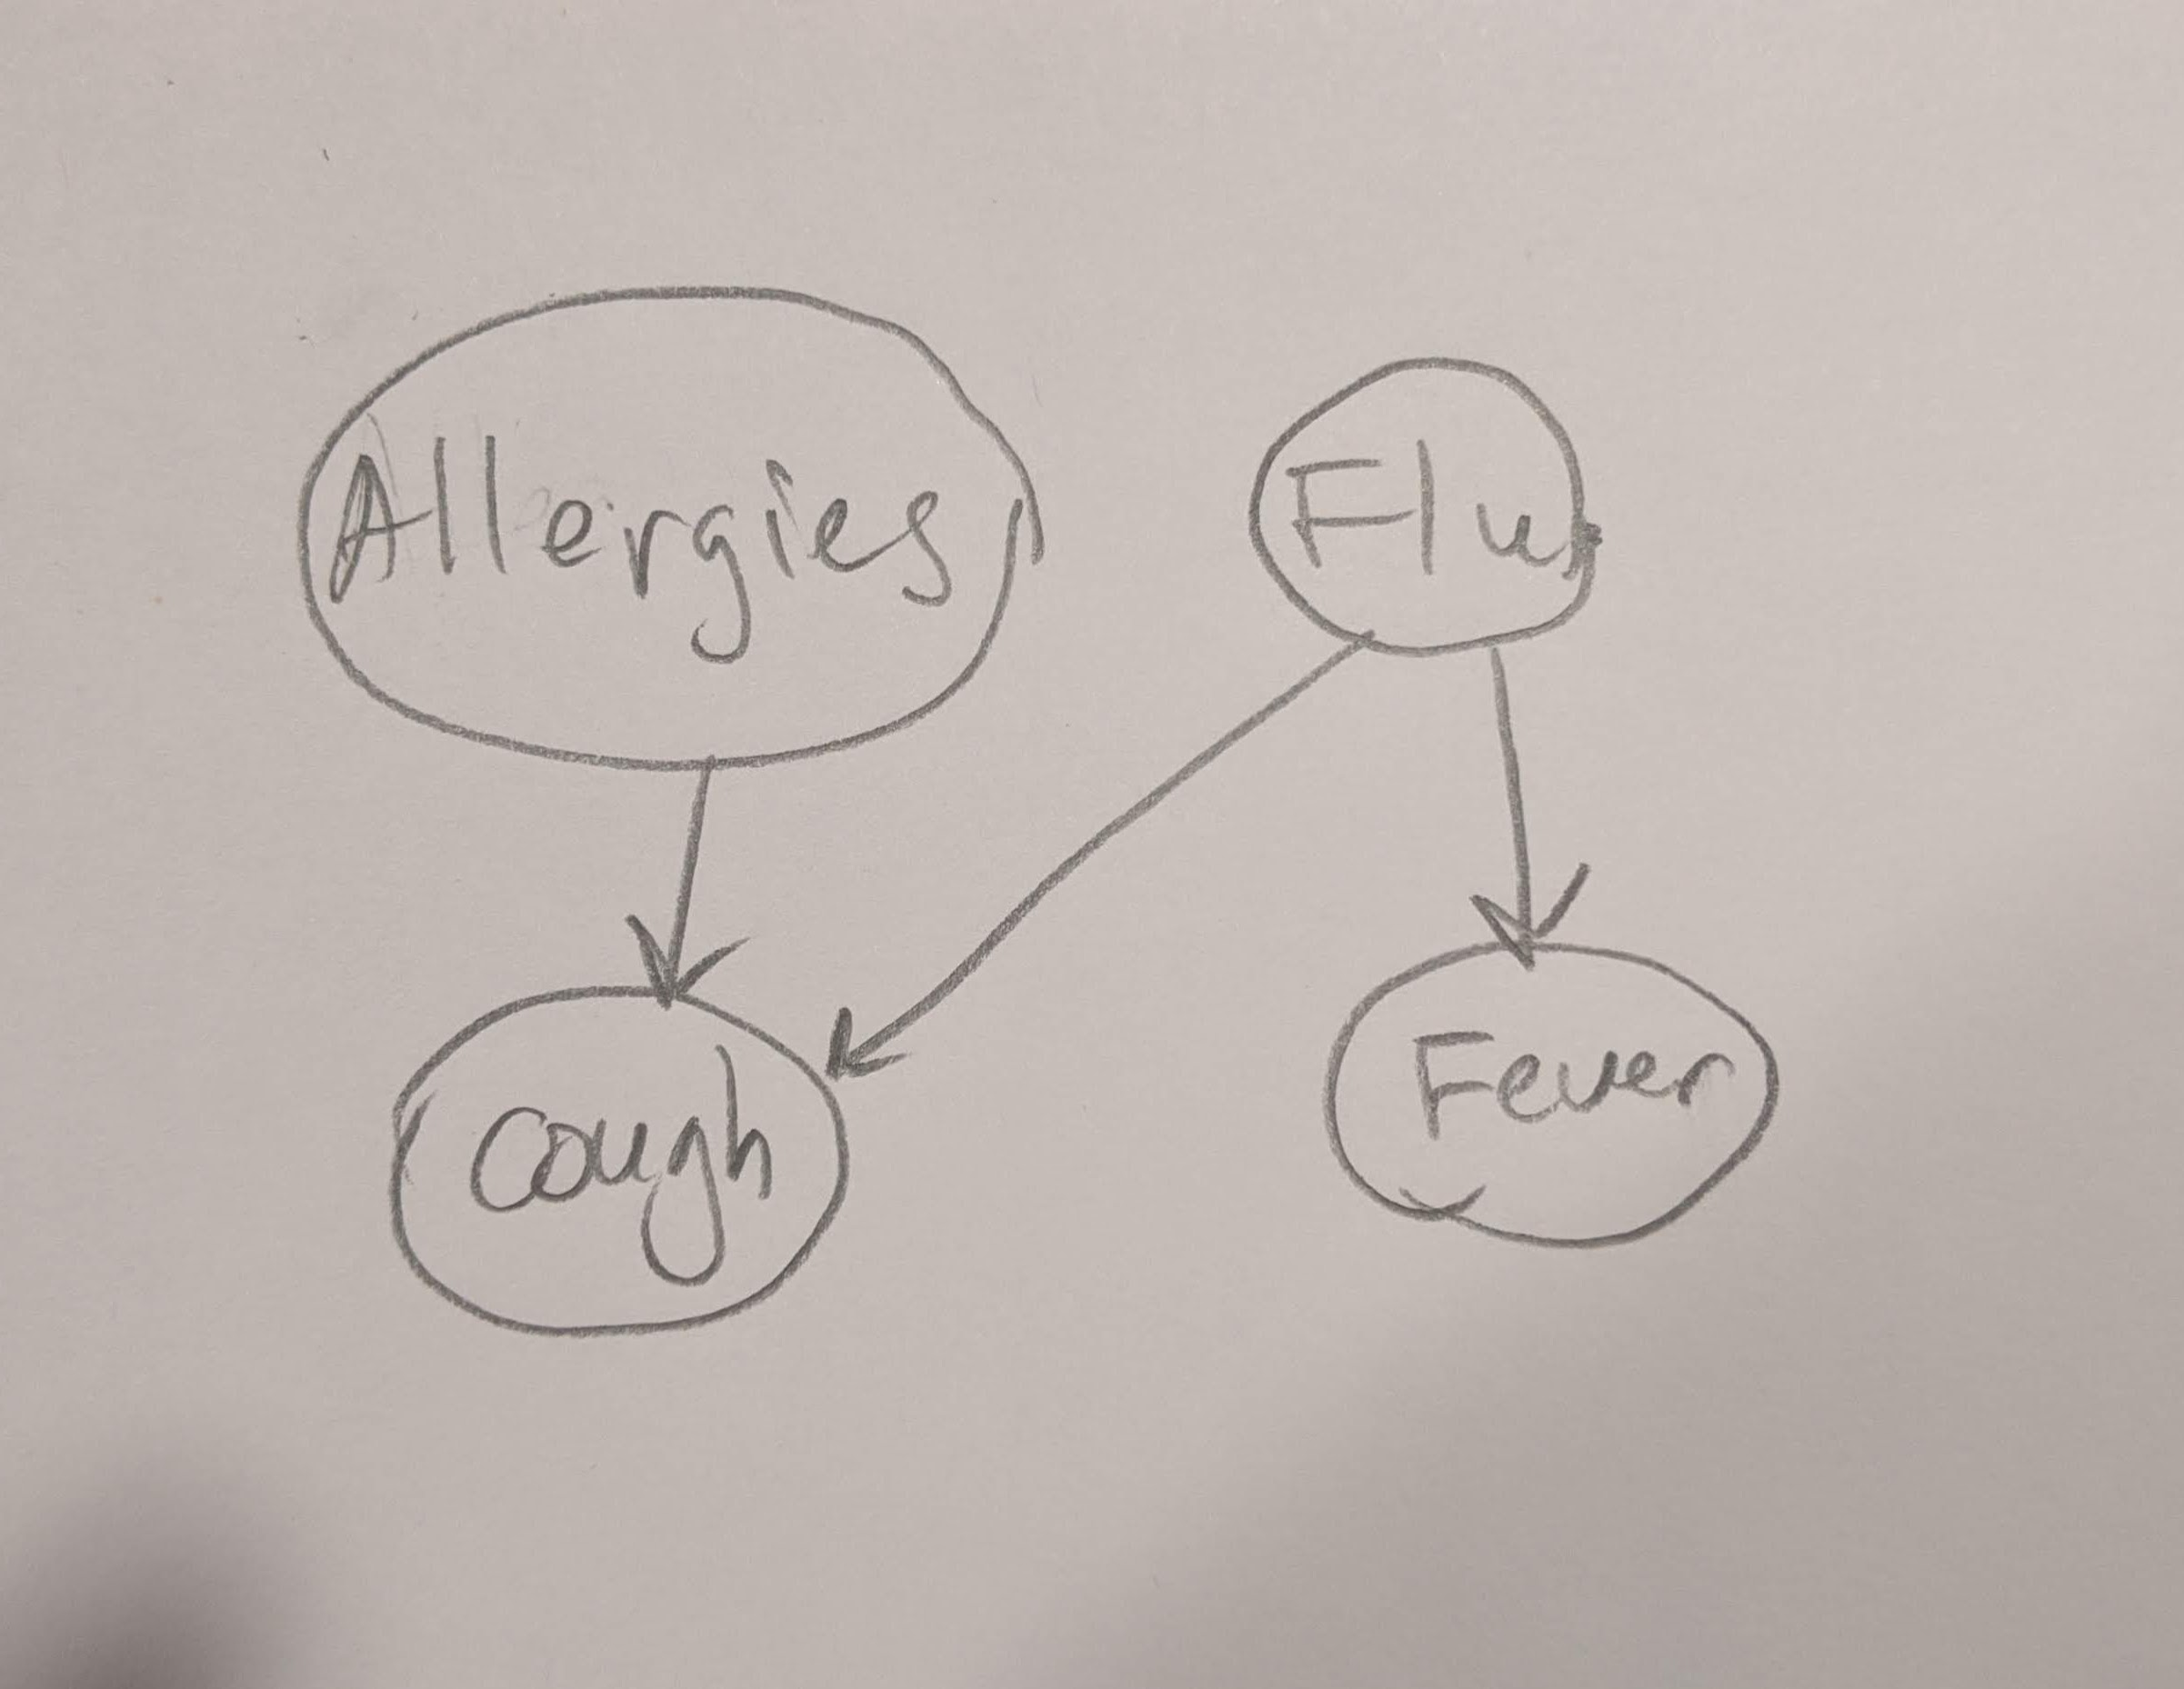
\includegraphics[width=0.45\textwidth]{3a}
    \item $p(cough,fever,allergy,flu) = p(cough\vert allergy,flu)p(fever\vert flu)p(allergy)p(flu)$
    \item Transition: $p(Z_t=k\vert Z_{t-1},u_t=i)$ \\
    Observation: $p(Y_t=l\vert Z_t=j,u_t=i)$ \\
    Prior: $p(Z_0=j)=\Pi_j$
    \item Consider the probability dsitributions below: \\ 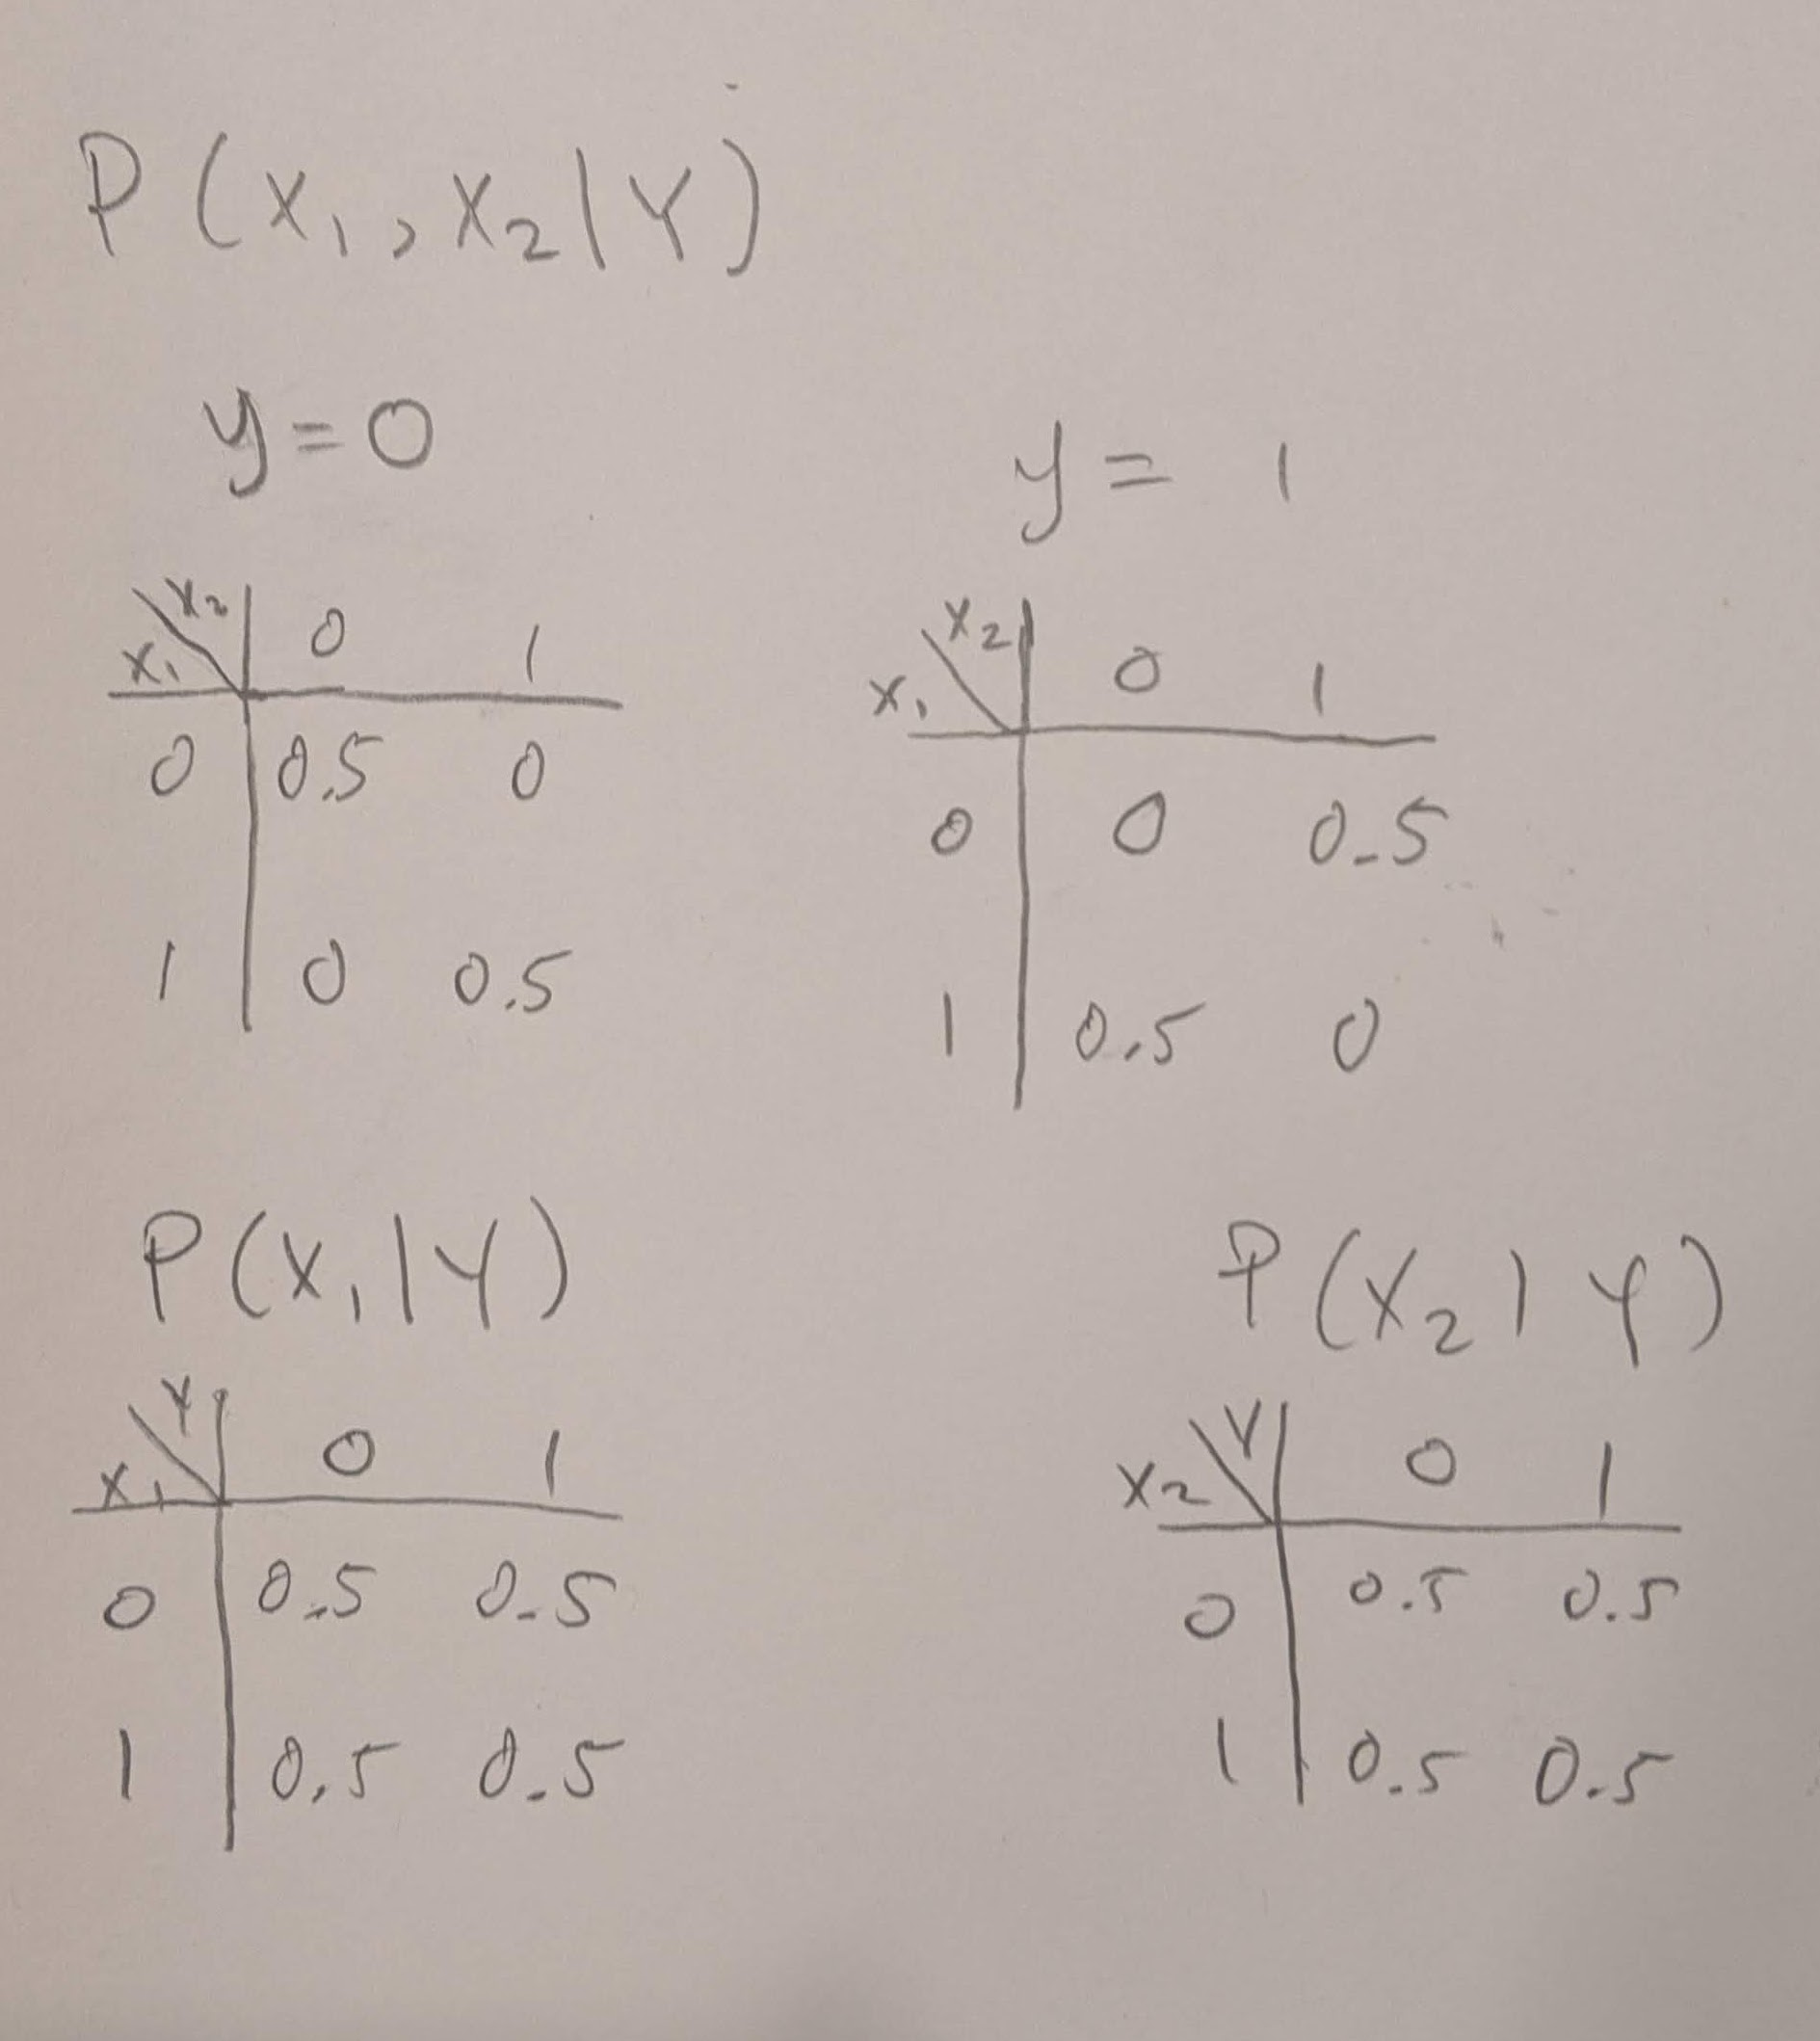
\includegraphics[width=0.4\textwidth]{3d} \\
    Explantion of probability dsitributions: \\
    Given $y = 0$, the two possible combinations of $(x_1, x_2)$ are $[(0,0), (1,1)]$. \\
    Given $y = 1$, the two possible combinations of $(x_1, x_2)$ are $[(0,1), (1,0)]$.\\
    Given $y=1$ $x_1$ can be either 0 or 1. Given $y=0$ $x_2$ can be either 0 or 1. \\
    Thus let $x_1 = 0, x_2 = 1, y=1 \rightarrow p(x_1,x_2 \vert y) = p(0,1 \vert 1) = 0.5$ \\
    $p(x_1 \vert y) = p(0 \vert 1) = 0.5$ \\
    $p(x_2 \vert y) = p(1 \vert 1) = 0.5$ \\
    $\rightarrow p(x_1 \vert y)p(x_2 \vert y) = p(0 \vert 1)p(1 \vert 1) = 0.5 * 0.5 = 0.25 \rightarrow p(x_1,x_2 \vert y) \neq p(x_1 \vert y)p(x_2 \vert y)$
\end{enumerate}
\end{enumerate}

\end{document}

